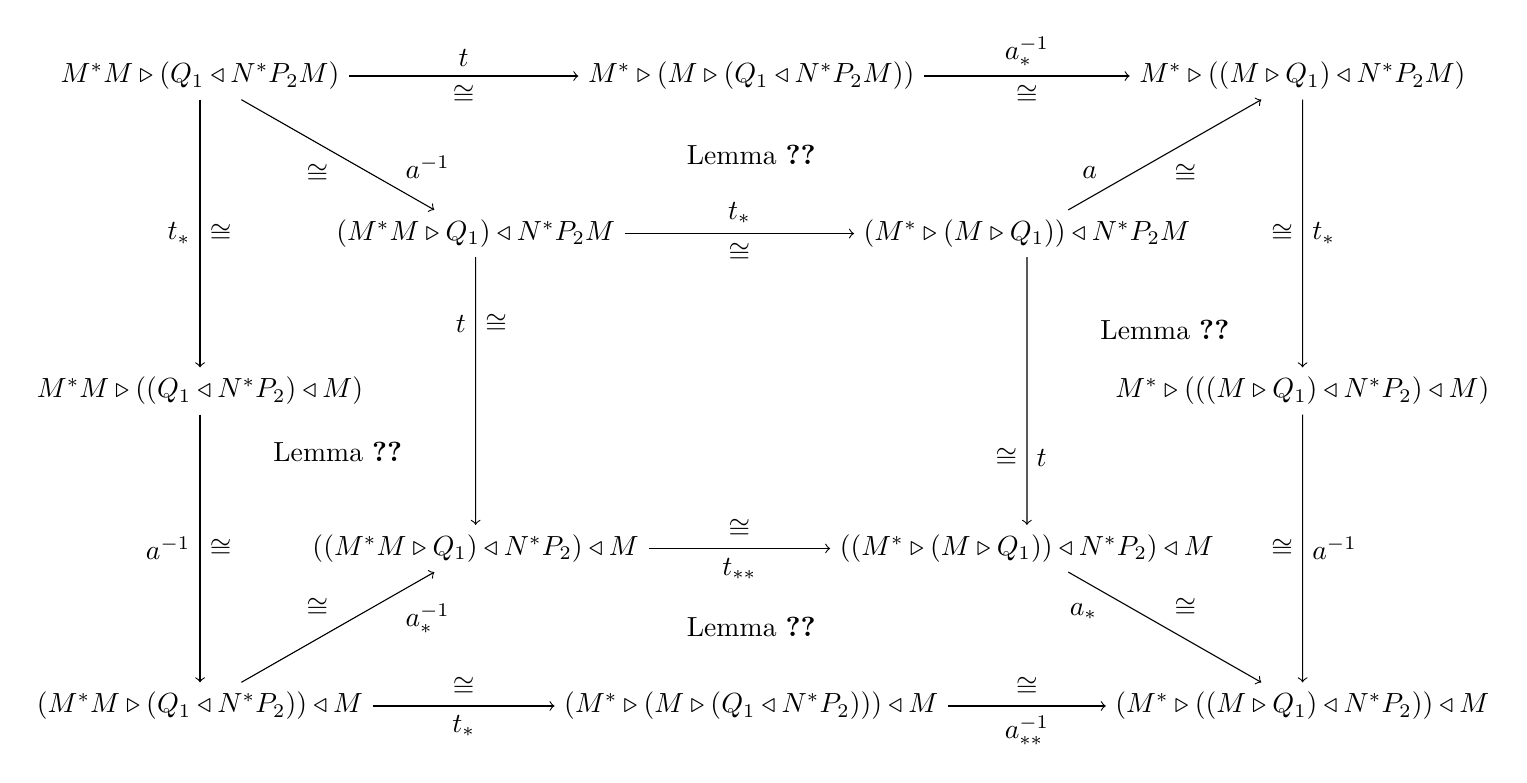
\begin{tikzpicture}[xscale=3.5, yscale=2]
	\node(F2) at (0, 4){$\lsh{M^*M \triangleright (Q_1 \triangleleft N^*P_2M)}$};
	\node(G2) at (2, 4){$\lsh{M^* \triangleright (M \triangleright (Q_1 \triangleleft N^*P_2M))}$};
	\node(H2) at (4, 4){$\lsh{M^* \triangleright ((M \triangleright Q_1) \triangleleft N^*P_2M)}$};
	\node(L2) at (0, 2){$\lsh{M^*M \triangleright ((Q_1 \triangleleft N^*P_2) \triangleleft M)}$};
	\node(M2) at (4, 2){$\lsh{M^* \triangleright (((M \triangleright Q_1) \triangleleft N^*P_2) \triangleleft M)}$};
	\node(Q2) at (0, 0){$\lsh{(M^*M \triangleright (Q_1 \triangleleft N^*P_2)) \triangleleft M}$};
	\node(R2) at (2, 0){$\lsh{(M^* \triangleright (M \triangleright (Q_1 \triangleleft N^*P_2))) \triangleleft M}$};
	\node(S2) at (4, 0){$\lsh{(M^* \triangleright ((M \triangleright Q_1) \triangleleft N^*P_2)) \triangleleft M}$};
	\node(W2) at (1, 3){$\lsh{(M^*M \triangleright Q_1) \triangleleft N^*P_2M}$};
	\node(Z2) at (3, 3){$\lsh{(M^* \triangleright (M \triangleright Q_1)) \triangleleft N^*P_2M}$};
	\node(A3) at (1, 1){$\lsh{((M^*M \triangleright Q_1) \triangleleft N^*P_2) \triangleleft M}$};
	\node(B3) at (3, 1){$\lsh{((M^* \triangleright (M \triangleright Q_1)) \triangleleft N^*P_2) \triangleleft M}$};

	\draw [->] (F2) -- node[above]{$\lsh{t}$} node[below]{$\cong$} (G2);
	\draw [->] (G2) -- node[above]{$\lsh{a^{-1}_*}$} node[below]{$\cong$} (H2);
	\draw [->] (H2) -- node[right]{$\lsh{t_*}$} node[left]{$\cong$} (M2);
	\draw [->] (M2) -- node[right]{$\lsh{a^{-1}}$} node[left]{$\cong$} (S2);
	\draw [->] (F2) -- node[left]{$\lsh{t_*}$} node[right]{$\cong$} (L2);
	\draw [->] (L2) -- node[left]{$\lsh{a^{-1}}$} node[right]{$\cong$} (Q2);
	\draw [->] (Q2) -- node[below]{$\lsh{t_*}$} node[above]{$\cong$} (R2);
	\draw [->] (R2) -- node[below]{$\lsh{a^{-1}_{**}}$} node[above]{$\cong$} (S2);

	\draw [->] (W2) -- node[above]{$\lsh{t_*}$} node[below]{$\cong$} (Z2);
	\draw [->] (W2) -- node[left, pos=0.25]{$\lsh{t}$} node[right, pos=0.25]{$\cong$} (A3);
	\draw [->] (Z2) -- node[right, pos=0.75]{$\lsh{t}$} node[left, pos=0.75]{$\cong$} (B3);
	\draw [->] (A3) -- node[below]{$\lsh{t_{**}}$} node[above]{$\cong$} (B3);
	\draw [->] (F2) -- node[above right, pos=0.8]{$\lsh{a^{-1}}$} node[below left]{$\cong$} (W2);
	\draw [->] (B3) -- node[below left, pos=0.2]{$\lsh{a_*}$} node[above right]{$\cong$} (S2);
	\draw [->] (Z2) -- node[above left, pos=0.2]{$\lsh{a}$} node[below right]{$\cong$} (H2);
	\draw [->] (Q2) -- node[below right, pos=0.8]{$\lsh{a^{-1}_*}$} node[above left]{$\cong$} (A3);

	\node at (barycentric cs:F2=1,H2=1,W2=1,Z2=1){Lemma \ref{lem:pentagon_a_and_t_2}};
	\node at (barycentric cs:A3=1,B3=1,Q2=1,S2=1){Lemma \ref{lem:pentagon_a_and_t_2}};
	\node at (barycentric cs:A3=1.7,F2=1,Q2=1.7,W2=1){Lemma \ref{lem:pentagon_a_and_t_2}};
	\node at (barycentric cs:H2=1.7,Z2=1.7,B3=1,S2=1){Lemma \ref{lem:pentagon_a_and_t_2}};
\end{tikzpicture}
